\chapter{Monitoraggio e controllo}
\label{ch:monitoraggio-e-controllo}

Il progetto è stato gestito col supporto di \emph{GitHub Projects}~\cite{cit:github-projects}. Questo strumento si integra con il DVCS Git utilizzato dal team e permette di gestire le attività di sviluppo in modo agile.
Inoltre, è stata prestata grande attenzione ad automatizzare il più possibile queste attività per ridurre al minimo il tempo necessario per la loro esecuzione e permettere agli sviluppatori di concentrarsi sui problemi di business.

\section{Reporting automatico}
\label{sec:reporting-automatico}

Ogni task dello sprint viene convertito in una GitHub issue~\cite{cit:github-issues} che ne riporta le dipendenze e le informazioni di base; un esempio di tale issue è riportato in \Cref{fig:issue-example}. Come mostrato in figura, il vantaggio di tale approccio sta nella possibilità di automatizzare il reporting delle attività svolte durante lo sprint. Infatti, un bot può analizzare i diversi task e calcolare quanti sono stati conclusi o meno per fare un report dell'andamento.

Grazie alla stretta integrazione fra il sistema di reporting e il DVCS, il programmatore non dovrà occuparsi di gestire alcun overhead dato che gli sarà sufficiente chiudere una issue per segnalare che il task corrispondente è stato completato.

\begin{figure}[htp]
  \centering
  \includegraphics[width=\textwidth]{images/task-example.png}
  \caption{Esempio di issue}
  \label{fig:issue-example}
\end{figure}

\subsection{Sprint burndown chart}
Inoltre, ad ogni sprint viene generato automaticamente uno \emph{sprint burndown chart} a partire dalle issue chiuse. Questo grafico viene aggiornato al completamento dei task e consente di monitorare lo stato di avanzamento dello sprint in tempo reale permettendo di avere un \emph{current period reporting} efficace.
È uno strumento fondamentale che permette di individuare rapidamente dei ritardi sulla tabella di marcia permettendo al team di analizzarne le cause tempestivamente.

Come mostrato in \Cref{fig:sprint-burndown-chart}, il grafico riporta sull'asse delle ascisse il giorno dello sprint e sull'asse delle ordinate l'effort rimanente. Inflessioni del grafico indicano ritardi o avanzamenti rispetto alla tabella di marcia ideale.

\begin{figure}[htp]
  \centering
  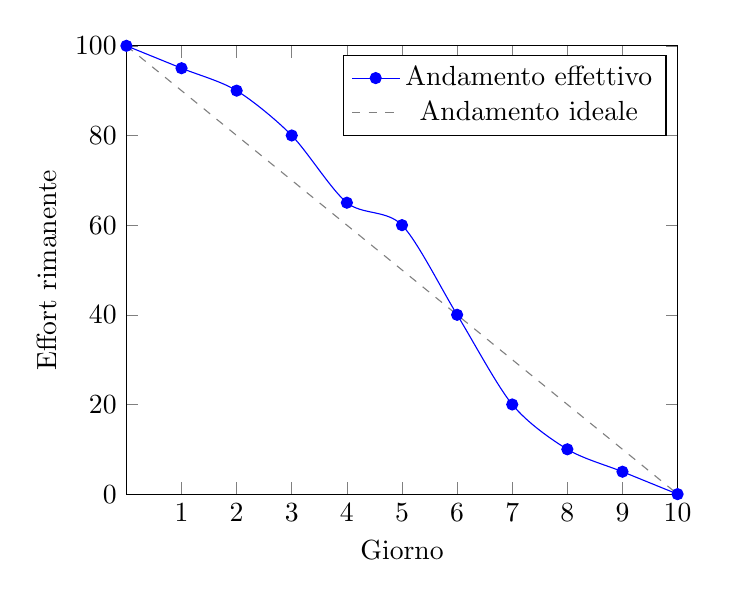
\begin{tikzpicture}
    \begin{axis}[
        xlabel={Giorno},
        ylabel={Effort rimanente},
        xmin=0, xmax=10,
        x=0.7cm,
        ymin=0, ymax=100,
        xtick={1,...,10},
        ytick={0,20,...,100}]
      \addplot[smooth,mark=*,blue] plot coordinates {
          (0,100)
          (1,95)
          (2,90)
          (3,80)
          (4,65)
          (5,60)
          (6,40)
          (7,20)
          (8,10)
          (9,5)
          (10,0)
        };
      \addlegendentry{Andamento effettivo}

      \addplot[dashed,color=gray,mark=none]
      plot coordinates {
          (0,100)
          (10,0)
        };
      \addlegendentry{Andamento ideale}
    \end{axis}
  \end{tikzpicture}
  \caption{Esempio di sprint burndown chart}
  \label{fig:sprint-burndown-chart}
\end{figure}

\subsection{Project Burndown Chart}
Per avere \emph{cumulative reporting} è stato anche realizzato un \emph{project burndown chart} che mostra lo stato di avanzamento dell'intero progetto.
Anche in questo caso il grafico viene generato automaticamente a partire dalle issue chiuse e permette di monitorare l'intero progetto.
Come mostrato in \Cref{fig:project-burndown-chart}, il grafico riporta gli sprint sull'asse delle ascisse e il numero di story point rimanenti sull'asse delle ordinate.

Questo strumento è fondamentale per poter stimare la velocità di sviluppo del team nel consumare story points. Infatti, per stimare il numero di story points da realizzare in uno sprint devono essere tenute in considerazione le storie concluse in precedenza ed eventuali difficoltà del team nel portarle a compimento.
Così facendo è possibile mantenere una velocità di sviluppo all'incirca costante per poter stimare con maggior precisione le tempistiche di consegna del progetto.

\begin{figure}[htp]
  \centering
  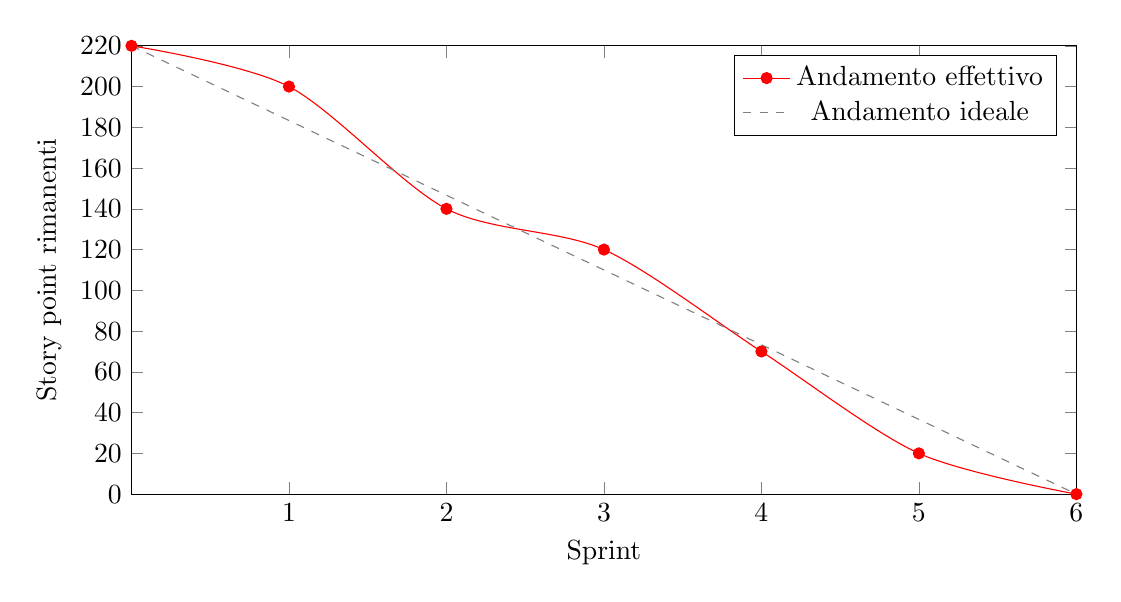
\begin{tikzpicture}
    \begin{axis}[
        xlabel={Sprint},
        ylabel={Story point rimanenti},
        xmin=0, xmax=6,
        x=2cm,
        ymin=0, ymax=220,
        xtick={1,...,6},
        ytick={0,20,...,220}]
      \addplot[smooth,mark=*,red] plot coordinates {
          (0,220)
          (1,200)
          (2,140)
          (3,120)
          (4,70)
          (5,20)
          (6,0)
        };
      \addlegendentry{Andamento effettivo}

      \addplot[dashed,color=gray,mark=none]
      plot coordinates {
          (0,220)
          (6,0)
        };
      \addlegendentry{Andamento ideale}
    \end{axis}
  \end{tikzpicture}
  \caption{Project burndown chart}
  \label{fig:project-burndown-chart}
\end{figure}

\subsection{Issue log}
Per mantenere traccia di tutte le problematiche incontrate durante lo svolgimento del progetto si è tenuto un issue log sfruttando le GitHub Issues: in questo modo, è possibile tracciare automaticamente i problemi e collegarli ai commit che ne implementano le soluzioni.
Le informazioni riportate per ogni issue sono:
\begin{itemize}
  \item Identificativo numerico
  \item Nome del problema
  \item Descrizione del problema
  \item Eventuale discussione su proposte risolutive
\end{itemize}

Un esempio di issue è riportato alla \Cref{fig:issue-example}.

\begin{figure}[htp]
  \centering
  \includegraphics[width=\textwidth]{images/issue-example.png}
  \caption{Esempio di issue: il numero è quello assegnato automaticamente da GitHub, il \emph{problem owner} è l'assegnatario della issue (in questo caso Nicolas) e lo stato di avanzamento viene tracciato automaticamente quando lo issue viene chiusa}
  \label{fig:issue-log}
\end{figure}

\section{Esempio di sprint}
In seguito è riportato come esempio lo svolgimento del terzo sprint con l'obiettivo di esemplificare il processo di stesura dello sprint e mostrare come sono state gestite situazioni eccezionali durante lo svolgimento del progetto.

\subsection{Descrizione degli sprint precedenti}
\subsubsection{Primo sprint}
Il primo sprint è stato dedicato al completamento della storia \href{user-story:i2-e4-u1}{I2-E4-U1} che aveva massima priorità e secondo le stime avrebbe impiegato lo sforzo di tutto il team di sviluppo.

Il vantaggio dell'avere una sola storia, comunque scomposta in numerosi task, è stato nel fatto che i membri del gruppo hanno potuto anche trovare il tempo di prendere confidenza con una metodologia di sviluppo a loro poco familiare. Infatti, il progetto è stato sviluppato utilizzando un'architettura funzionale con meccanismi di programmazione funzionale avanzata.
Per questo motivo è stato necessario per Giacomo -- già esperto nel settore -- fare qualche corso di formazione per i propri colleghi e supportarli durante lo sviluppo.

In questo modo, durante lo sprint, Giacomo ha svolto \emph{pair programming} con i propri 4 colleghi per poterli aiutare.

\subsubsection{Secondo sprint}
Nel secondo sprint il team -- forte della maggior esperienza acquisita nel primo sprint -- ha aumentato il numero di story points da completare.
Inoltre, poiché Giacomo non ha più dovuto supportare attivamente in \emph{pair programming} i propri colleghi, ha potuto dedicarsi interamente al completamento di nuovi task.

Per questo motivo lo sprint è stato concluso con un ottimo risultato di 60 story points.

\subsection{Pianificazione dello sprint}
Durante la retrospettiva dello sprint precedente si è osservato come, pur essendo possibile completare 60 story points in uno sprint, questo abbia comportato una riduzione nel tempo slack che poteva essere dedicato alla gestione di possibili imprevisti. Perciò si è stabilito di ridurre gli story points dello sprint a 50; questo permette comunque di consegnare il MVP entro la scadenza prestabilita mantenendo un ambiente di lavoro più rilassato e produttivo.

Le storie che si è scelto di includere nello sprint, per un totale di 49 punti, sono le seguenti:
\begin{itemize}
  \item \href{user-story:i2-e4-u2}{I2-E4-U2} (7 punti)
  \item \href{user-story:i2-e4-u4}{I2-E4-U4} (5 punti)
  \item \href{user-story:i2-e4-u9}{I2-E4-U9} (5 punti)
  \item \href{user-story:i2-e4-u3}{I2-E4-U3} (2 punti)
  \item \href{user-story:i1-e1-u1}{I1-E1-U1} (20 punti)
  \item \href{user-story:i1-e2-u1}{I1-E2-U1} (1 punto)
  \item \href{user-story:i1-e2-u2}{I1-E2-U2} (1 punto)
  \item \href{user-story:i1-e2-u3}{I1-E2-U3} (3 punti)
  \item \href{user-story:i1-u1}{I1-U1} (5 punti)
\end{itemize}
\todo[inline]{i link delle user stories sono rotti}
\todo[inline]{mettere il link all'appendice}

\subsection{Retrospettiva}
Durante lo sprint si è verificata una situazione eccezionale che ha comportato un ritardo nello sviluppo:
il primo weekend dello sprint Nicolò ha chiesto una settimana di malattia.

L'assenza di Nicolò non è stata tanto lunga da compromettere lo sviluppo e rendere necessario lo spostamento di risorse da altri progetti di Atedeg.
Il problema è stato affrontato come già prestabilito nella strategia di mitigazione del rischio: si è rimodulato lo sprint backlog in maniera tale da bilanciare il carico di lavoro fra i programmatori rimanenti. Inoltre, dato che nella realizzazione dello sprint si era già considerato un certo \emph{slack} per gli sviluppatori, questi hanno potuto coprire parzialmente il lavoro lasciato da Nicolò.

In \Cref{fig:burndown-sprint-3} è riportato lo sprint burndown chart che mostra come al giorno 6 (il primo lunedì di lavoro dopo la notifica di malattia da parte di Nicolò) l'effort rimanente sia stato ridotto rimandando dei task allo sprint successivo.
Si è contattato il cliente per comunicargli dell'accaduto e stabilire quali user story avessero minore importanza e ottenere l'approvazione nel ritardare la consegna di queste. Perciò si è stabilito di comune accordo di mantenere nello sprint i task relativi alla realizzazione dell'e-commerce rimandando invece quelli relativi alla pianificazione automatica.
In questo modo si è riuscito a consegnare in tempo il MVP richiesto con soddisfazione del cliente.
\todo[inline]{Dire esplicitamente che l'MVP in questo caso è il sito di e-commerce funzionante perché possa essere usato dai clienti entro settembre}

\begin{figure}[htp]
  \centering
  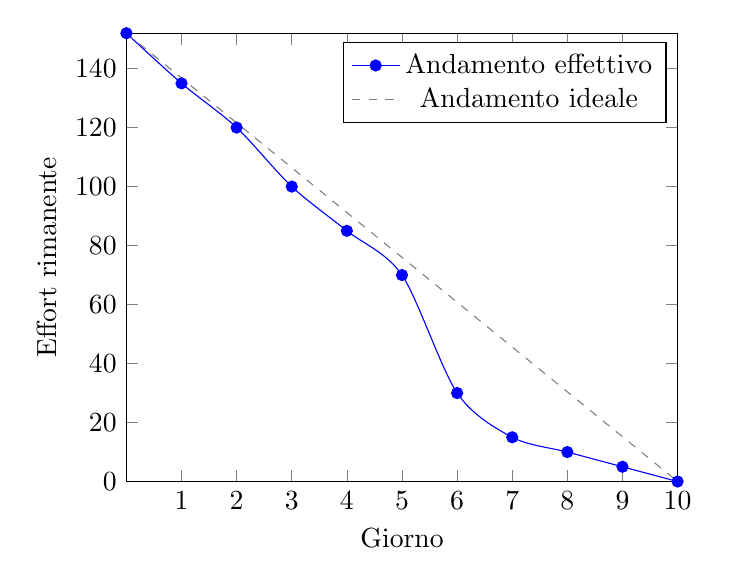
\begin{tikzpicture}
    \begin{axis}[
        xlabel={Giorno},
        ylabel={Effort rimanente},
        xmin=0, xmax=10,
        x=0.7cm,
        ymin=0, ymax=152,
        xtick={1,...,10},
        ytick={0,20,...,152}]
      \addplot[smooth,mark=*,blue] plot coordinates {
          (0,152)
          (1,135)
          (2,120)
          (3,100)
          (4,85)
          (5,70)
          (6,30)
          (7,15)
          (8,10)
          (9,5)
          (10,0)
        };
      \addlegendentry{Andamento effettivo}

      \addplot[dashed,color=gray,mark=none]
      plot coordinates {
          (0,152)
          (10,0)
        };
      \addlegendentry{Andamento ideale}
    \end{axis}
  \end{tikzpicture}
  \caption{Sprint burndown chart del terzo sprint}
  \label{fig:burndown-sprint-3}
\end{figure}


